\chapter{Estrategia Empírica}

\noindent En este capítulo, analizo el impacto que tuvieron las cámaras de velocidad del programa de fotocívicas sobre la seguridad vial en la Ciudad de México. En particular, estudio cómo la instalación de estos radares afecta el número, la tasa y la severidad de los incidentes viales, poniendo especial énfasis en los accidentes con lesionados y con víctimas fatales. A partir de la literatura revisada, planteo la hipótesis de que las cámaras generan una reducción de estos incidentes en el entorno inmediato donde operan, aproximadamente en un radio de 300 metros alrededor de cada dispositivo.\\

Para poner a prueba esta hipótesis, construyo distintas áreas de influencia en torno a las cámaras y evalúo sus efectos utilizando dos enfoques complementarios: propensity score matching y modelos de diferencia en diferencias con información de incidentes viales proveniente del C5. En las secciones que siguen, primero presento el marco conceptual que motiva mis hipótesis y los mecanismos a través de los cuales los radares de velocidad podrían modificar la ocurrencia y gravedad de los accidentes. Después, explico cómo, a partir de este marco conceptual y de las características de los datos disponibles, llego a la estrategia de identificación final. Finalmente, hago explícitos los supuestos bajo los cuales mis resultados pueden interpretarse de manera causal y discuto el alcance y las limitaciones de esta interpretación.\\

\section{Marco Conceptual}
\subsection{Velocidad y dinámica del flujo vehicular}
\noindent Una de las vías más directas a través de la cuales las cámaras de velocidad pueden afectar la seguridad vial es modificando la velocidad a la que circulan los vehículos y, con ello, la dinámica del flujo vehicular en su entorno. A mayor velocidad aumenta tanto la probabilidad de que ocurra un siniestro como la severdidad del mismo, dado que el conductor tiene menos tiempo y distancia para reaccionar (García, 2018).\\

\indent Las cámaras de velocidad actúan precisamente sobre ese canal: generan un incentivo a reducir la velocidad, al aumentar la probabilidad percibida de sanción en un punto específico de la vialidad. Sin embargo, este efecto rara vez corresponde a una reducción uniforme de la velocidad a lo largo de un tramo completo, sino que más bien se traduce en lo que se conoce como el "efecto canguro": una disminución abrupta antes del radar de velocidad y una aceleración una vez que se ha salido del área de efectividad (Li et al., 2013 y 2020; Graham et al., 2019; Mountain et al., 2005; De Pauw et al., 2014).\\

En un contexto urbano como la Ciudad de México, es razonable anticipar dinámicas similares, que pueden tener impactos distintos en el número de incidentes. Por un lado, la reducción de velocidad en el área de influencia puede disminuir los accidentes y su severidad al darle más tiempo de reacción y de frenado al conductor, y disminuyendo la severidad en caso de presentarse un incidente. Por otro lado, la forma en la que los conductores ajustan su comportamiento no es homogénea: no solo existe diferencia entre aquellos que respetan de manera estricta el límite de velocidad y aquellos que solo lo hacen cuando su riesgo de ser detectados es más alto, sino que recordemos que las sanciones en Ciudad de México tampoco son iguales para todos los conductores, y están sujetas a la placa de registro del vehículo. Esta heterogeneidad de respuestas genera cambios no solo en el nivel medio de velocidad, sino también en su variablidad.\\

En vías donde coexisten vehículos muy lentos con otros muy rápidos tienden a registrar mayores tasas de incidentes que vías donde todos los vehículos circulan a una velocidad similar (Aart, Schagen, 2005; Choudharya et al., 2018; Wang et al., 2018). Bajo este argumento, un esquema de control que induce a algunos conductores a frenar de manera brusca y a otros a mantener velocidades altas puede, localmente, aumentar el riesgo de choques por alcance, maniobras evasivas y conflictos entre carriles, aun cuando la velocidad promedio en el tramo se reduzca.\\ 

Es por ello importante que un análisis que busque analizar los efectos de las cámaras de velocidad debe hacerlo con especial atención a cambios en las inmediaciones más cercanas de los radares, así como elegir controles que capten las características del entorno vial y del flujo vehicular, de modo que sea posible aislar el efecto específico de la cámara de otros factores que influyen en la ocurrencia y severidad, así como evitar reportar datos tan extensos que no capturen efectos debido a la dilusión del impacto.\\ 

\subsection{Migración potencial de accidentes y ausencia de datos de flujo vehicular}
\noindent Una segunda vía a través de la cual las cámaras de velocidad pueden afectar el número y la severidad de los incidentes viales es mediante la migración de los accidentes asociada a cambios en las rutas de los conductores. La literatura documenta que es posible que la presencia de radares induzca a algunos usuarios a elegir vías alternativas para evitar el riesgo de sanción (Mountain, 2005; Li et al., 2013). En principio, controlar por el volumen de tráfico en el tramo permitiría distinguir si las variaciones en la siniestralidad se deben a cambios en la exposición al riesgo o a un efecto real de las cámaras. Sin embargo, en contextos donde no es posible acceder a información detallada de flujo vehicular ---como es el caso en la Ciudad de México---, la evaluación de efectos en áreas, en lugar de limitarse al tramo puntual de la cámara, ofrece una forma de mitigar este problema hasta cierto punto (Li et al., 2020; Christie et al., 2003).\\

\indent Cambios en las trayectorias pueden tener varias consecuencias simultáneas. Por un lado, podrían modificar el flujo vehicular tanto en la vía con la cámara como en calles aledañas, liberando parcialmente la primera y concentrando vehículos en las segundas. Por otro lado, la composición vehicular de los conductores en cada ruta también puede alterarse: usuarios más aversos al riesgo o más sensibles a las multas podrían evitar de forma sistemática los corredores con radares de velocidad, mientras que conductores menos aversos seguirían transitando por esas vías.\\

En ausencia de datos de flujo vehicular que nos permitan estuidar variaciones en las inmediaciones de los radares de velocidad, es necesario encontrar una forma de capturar estas posibles redistribuciones de tráfico, ya que de no hacerlo, podría confundirse una simple reasignación espacial de los accidentes con una reducción genuina del riesgo. Evaluar el impacto de las cámaras a nivel de áreas de influencia que incluyan tanto el entorno inmediato del radar como sus proximidades ayuda a incorporar, al menos parcialmente, los siniestros que pudieran estar desplazándose hacia calles cercanas.\\

\subsection{Ventana temporal de análisis}
\noindent Para determinar el horizonte temporal de análisis es necesario equilibrar tres consideraciones: capturar con suficiente detalle la dinámica previa a la intervención; observar la evolución de sus efectos una vez implementada; y limitar el horizonte para que los periodos que se comparan sigan siendo razonablemente homogéneos entre sí. La literatura sobre cámaras de velocidad se mueve justamente dentro de ese equilibrio. Por un lado, evita tratarlas como intervenciones de efecto permanente e inmutable; en su lugar, define ventanas de tiempo finitas y comparables. Li et al. (2013) fijan un periodo 1999–2007 que, para cada sitio, garantiza tres años de información antes y tres después de la instalación, y dentro de ese marco analizan distintas bandas espaciales. En un trabajo posterior, Li et al. (2020) mantienen la idea de un bloque pretratamiento de tres años, pero prestan especial atención a la evolución del efecto: dividen los doce años posteriores en ventanas de igual longitud, precisamente para no mezclar en una sola estimación periodos que pueden tener comportamientos distintos, y efectivamente encuentran que el impacto se va diluyendo con el paso del tiempo. Christie et al. (2003) siguen una lógica similar al trabajar con una serie 1996–2000 y definir periodos before–after de varios años para estabilizar las tasas locales de choques en cada banda.\\

La comparación sistemática que hacen Li et al. (2013) de distintos estudios muestra que la elección del horizonte responde a objetivos analíticos distintos, más que a una regla única sobre qué ventana es correcta. Horizontes muy largos ---de hasta diez años de choques como Hess y Polak (2003) o Newstead y Cameron (2003)--- son útiles cuando se busca modelar con detalle tendencias de fondo. En el otro extremo, trabajo con ventanas muy cortas, del orden de un año y medio en total, como Shin et al. (2009), son adecuados para capturar cambios casi inmediatos tras la instalación de los radares, aún a costa de una mayor variabilidad por fluctuaciones viales. Entre estos dos extremos, los estudios que intentan evaluar efectos locales y relativamente estables en el tiempo tienden a converger en esquemas de tres años antes y tres años después de la instalación (Mountain et al, 2004, 2005; Gains et al., 2004, 2005; Li et al., 2013). Dado que mi objetivo es precisamente identificar el efecto local de las cámaras, controlando por tendencias generales sin comparar contextos que sean muy distintos entre sí, una ventana simétrica de tres años previos y tres años posteriores resulta la opción más adecuada.

Cabe destacar que esta ventana de tres años y tres años después enfrenta un reto crucial: abarca el perido de la pandemia por Covid-19, que alteró de manera drástica los patrones de movilidad. A partir de marzo de 2020, las restricciones sanitarias y el confinamiento redujeron de forma importante los desplazamientos diarios. De acuerdo con la Secretaría de Movilidad (SEMOVI, 2024), el Sistema de Movilidad Integrada registró una disminución del 45\% en el tránsito vehicular respecto a los niveles previos a la pandemia. Como era de esperarse, esto se tradujo en una caída en el número total de incidentes viales, pero también lo hizo en un aumento en su severidad, atribuido por la SEMOVI a menores niveles de congestión que facilitaban el tránsito a velocidades más altas. Si no se corrige por este choque exógeno en la movilidad, cualquier estimación del efecto de las fotocívicas correría el riesgo de confundir la plítica y los cambios en patrones de movilidad.\\

Como ya se adelantaba, la ausencia de datos detallados de flujo vehicular en las inmediaciones de cada cámara agrava este problema, pues impide controlar directamente la exposición al riesgo en cada tramo. Sin embargo, fue posible construir medidas de movilidad de referencia que permiten aproximar estas dinámicas y mitigar el sesgo potencial. Por un lado, se cuenta con datos de los radares de conteo permanentes instalados en las casetas de peaje en las periferias de la ciudad, que capturan la evolución del flujo vehicular de entrada y salida del área metropolitana a lo largo del periodo de estudio. Por otro lado, se dispone de información sobre la afluencia en estaciones del Metro, que funcionan como un indicador complementario de la movilidad cotidiana en distintos puntos de la ciudad.\\

En la estrategia empírica, estas series se incorporan como controles que varían en el tiempo y, en la medida de lo posible, se vinculan espacialmente con las áreas tratadas y de control. De este modo, aún cuando no se observa el flujo vehicular exacto en cada intersección, sí pueden captarse las oscilaciones en la movilidad general.

\section{Identificación de supuestos y selección de la muestra}
\subsection{Independencia condicional}
\noindent Para evaluar si las cámaras de velocidad tuvieron un efecto causal en el número o severidad de incidentes viales, el supuesto de indepenciencia condicional debe satisfacerse: condicionando en un conjunto adecuado de covariables observables, la decisión de instalar una cámara de velocidad en un área dada es “tan buena como aleatoria” con respecto a los resultados de seguridad vial que se analizan (número y severidad de incidentes). Bajo este supuesto, cualquier diferencia sistemática en las zonas con y sin cámara, una vez controladas las covariables, puede interpretarse como un efecto causal atribuible a la instalación del dispositivo y no a otros factores no observados. (Angrist and Pischke, 2009).\\

En la práctica, la asignación de cámaras de velocidad dista de ser aleatoria. En particular, durante la implementación del programa de Fotocívicas, las autoridades reubicaron los radares hacia tramos caracterizados por mayor incidencia de hechos de tránsito, poniendo especial énfasis en aquellos con más personas muertas y lesionadas, así como en puntos con altos volúmenes de tránsito y donde el límite de velocidad se incumplía con mayor frecuencia (SEMOVI, 2019). Es decir, los tramos tratados ya eran, antes de la instalación, sistemáticamente más riesgosos que los no tratados. Una comparación directa entre ambos grupos sin un ajuste cuidadoso heredaría este sesgo de selección y sobreestimaría, o subestimaría, el verdadero efecto de las cámaras.\\

\subsection{Tendencias paralelas}
\noindent La discusión del supuesto de independencia condicional deja claro por qué no es creíble comparar directamente cualquier área con cámara contra cualquier área sin cámara, y por qué es necesario construir un grupo de control comparable a partir de covariables observables. Sin embargo, como la estrategia final de esta tesis no se limita al emparejamiento, sino que combina \emph{propensity score matching} con diferencia en diferencias, hace falta introducir un supuesto adicional de naturaleza temporal: el de tendencias paralelas. En este contexto, dicho supuesto establece que, en ausencia del programa de Fotocívicas, la diferencia en siniestralidad entre las áreas tratadas y las áreas de control se habría mantenido estable a lo largo del tiempo. Esto no implica que ambos grupos deban partir del mismo nivel de accidentes; lo importante es que, sin intervención, hubieran seguido trayectorias similares. Bajo este supuesto, la evolución del grupo de control puede utilizarse como una aproximación del contrafactual del grupo tratado.\\

Este supuesto es especialmente relevante en este análisis porque el contrafactual de las áreas tratadas no es observable: una vez instaladas las cámaras, ya no es posible ver directamente qué habría ocurrido con esas mismas zonas si no hubieran recibido el tratamiento. El \emph{propensity score matching} ayuda a que la comparación sea más creíble al emparejar áreas con características observables similares, pero no sustituye el supuesto temporal que exige la diferencia en diferencias. En otras palabras, el matching mejora la comparabilidad inicial entre grupos, mientras que el supuesto de tendencias paralelas es el que permite usar la trayectoria de los controles emparejados como aproximación de lo que habría pasado con las áreas tratadas en ausencia del programa. Por ello, para interpretar de manera causal el coeficiente de interacción entre tratamiento y periodo posterior, es necesario mostrar que las trayectorias previas entre áreas tratadas y controles emparejados son razonablemente comparables.\\

\subsection{Restricciones de la muestra y construcción de las áreas de análisis}
\noindent La evaluación del efecto de las cámaras de velocidad exige definir con precisión el universo de estudio y la unidad espacial de análisis. En esta sección describo cómo se restringe la muestra y cómo se construyen las áreas tratadas y de control.\\

\textbf{Unidad de análisis}. Como ya se ha ido adelantando, en este caso la unidad de análisis corresponde a áreas circulares concéntricas en los radares de velocidad, sin embargo, conviene entender el primer enfoque que se tuvo para poder evaluar los beneficios de estas de forma más adecuada. Este primer enfoque consistió en superponer sobre la Ciudad de México una malla regular de celdas cuadradas. Cada celda que contenía al menos una cámara de velocidad se definía como \emph{área tratada}, mientras que las celdas sin cámaras se consideraban como posibles \emph{controles}. Para reducir la heterogeneidad entre celdas, se imponía además que cada celda tuviera traslape con alguna vía primaria de la ciudad.\\

Sin embargo, este enfoque resultó ser muy sensible a decisiones arbitrarias en la construcción de la malla. En particular, pequeñas variaciones en el \emph{offset} del grid (desplazamientos horizontales o verticales en el orden de 10 metros en la posición de origen) cambiaban la distancia entre las cámaras y el centro de sus respectivas celdas, lo que en algunos casos dejaba a la cámara muy cercana al borde de la celda y, por lo tanto, fuera del área donde se esperaría observar su efecto. Como consecuencia, estimaciones que eran estadísticamente significativas con una malla determinada dejaban de serlo con una ligera modificación del grid, aun manteniendo el mismo tamaño de celda. Se exploró una variante en la que se seleccionaba, para cada tamaño de celda, la malla que minimizara la distancia entre cada cámara y el centro de su celda, al tiempo que maximizara la longitud de vías primarias contenidas en cada celda. No obstante, los resultados seguían siendo poco robustos a cambios mínimos en la configuración del grid. Dado que esta falta de robustez cuestiona la credibilidad de las inferencias causales, descarté este enfoque.

Para superar estos problemas, opté por definir áreas de análisis centradas directamente en los puntos donde se ubican las cámaras de velocidad. En concreto, para cada cámara se construyen áreas circulares concéntricas con radios de 37.5, 50, 100, 150, 200 y 250 metros. Cada combinación cámara--radio define una posible \emph{área tratada}. Estos radios permiten estudiar cómo varía el efecto de las cámaras a distinta distancia del punto de control, siguiendo la práctica habitual en la literatura que analiza efectos locales de intervenciones puntuales sobre la seguridad vial. En la sección de resultados se presentan las estimaciones para cada radio por separado, lo que permite interpretar el impacto de las cámaras como una función continua de la distancia y no sólo en un punto arbitrario.\\

Con esta redefinición, la distancia al radar deja de depender de cómo se dibuja una malla y pasa a formar parte directa del análisis. Así, en lugar de comparar resultados que cambian por decisiones arbitrarias de partición espacial, es posible observar de manera más clara si el efecto se concentra cerca de la cámara o si se diluye conforme aumenta el radio.

En aquellos casos en los que los círculos de dos o más cámaras se traslapan para un mismo radio, se procede de la siguiente forma: se calcula el punto medio entre los pares de cámaras cuyos círculos se intersecan, y este punto medio se toma como nuevo centro del círculo para ese radio. El procedimiento se itera hasta obtener un único centro para cada área, evitando así contar dos veces zonas que están simultáneamente bajo la influencia de varias cámaras. El resultado final es un conjunto de áreas circulares tratadas, no solapadas entre sí para cada radio, que capturan de manera directa el entorno inmediato de las cámaras.\\

\textbf{Controles}. La definición de áreas tratadas resuelve el problema de robustez, pero plantea un nuevo reto: es necesario construir un universo de áreas comparables que puedan fungir como controles. Para cada radio considerado, y para cada círculo tratado, genero una \emph{vecindad de círculos candidatos a control} mediante el siguiente procedimiento: 

\begin{enumerate}
    \item Se mantiene fijo el centro del círculo tratado y su radio $r$ (por ejmplo, $r=100m$.
    \item Alrededor de este círculo, se construye una malla de círculos adicionales de radio $r$, dentro de un radio máximo de 12.5 km respecto al centro original.
    \item Se descartan todos los círculos que tengan traslape con otros círculos tratados
\end{enumerate}

No todas las áreas generadas mediante la malla de círculos son elegibles como controles. Con el objetivo de que las unidades tratadas y de control compartan un contexto vial similar, restrinjo el universo de estudio a aquellas áreas --tratadas y de control-- que presentan traslape con alguna vía primaria de la Ciudad de México.\\ 

Esta decisión se fundamenta en primer lugar, en las diferencias estructurales entre vías primarias y secundarias. La red vial de la Ciudad de México tiene una traza anular (Guía para el control de la velocidad, 2018), lo que deriva en vías primarias que concentran el flujo entre el centro y la periferia, operan a mayores velocidades, y dada la definición de traza anular, funcionan como ''barreras urbanas'' que separan barrios y colonias. Las vías secundarias y calles locales, en contraste, actúan principalmente como alimentadoras y desahogo hacia las primarias, con límites de velocidades menores y un entorno predominantemente residencial.\\

El propio marco normativo distingue explícitamente entre tipos de vía. El Artículo 9 del Reglamento de Tránsido de la Ciudad de México establece que, en ausencia de señalamiento específico, los límites generales de velocidad son crecientes con la jerarquía vial: 80 km/h en carriles centrales de vías de acceso controlado (fracción I), 50 km/h en vías primarias (fracción II) y 40 km/h en vías secundarias., incluyendo laterales de vías de acceso controlado (fracción III). en zonas de tránsito calmado el límite desciende a 30 km/h (fracción IV), minetras que en zonas escolares, de hospitales, asilos, la velocidad máxima es de 20 km/h (fracción V). El propio reglamento asume que las vías primarias y de acceso controlado operan a velocidades mayores, lo que sugiere también mayores niveles de exposición al riesgo vial.\\ 

La evidencia descriptiva es coherente con este diagnóstico. Utilizando una agregación espacial en hexágonos de aproximadamente 428 metros de largo (considerando la diagonal mayor), el promedio mensual de accidentes en el periodo previo al tratamiento (2016--2019) es de $2.36$ siniestros (desviación estándar de $1.4$) en hexágonos que contienen alguna vía primaria, frente a $1.33$ siniestros mensuales (desviación estándar de $0.36$) en aquellos que no cuentan con vías primarias. Las distribuciones de accidentes (Figura 2.2) muestran, además, colas más pesadas en las áreas con vías primarias, mientras que lás áreas sin ellas se concentran en valores bajos.\\

\begin{figure}
    \centering
    \caption{Promedio mensual de accidentes en la CDMX (2016 - 2019)}
    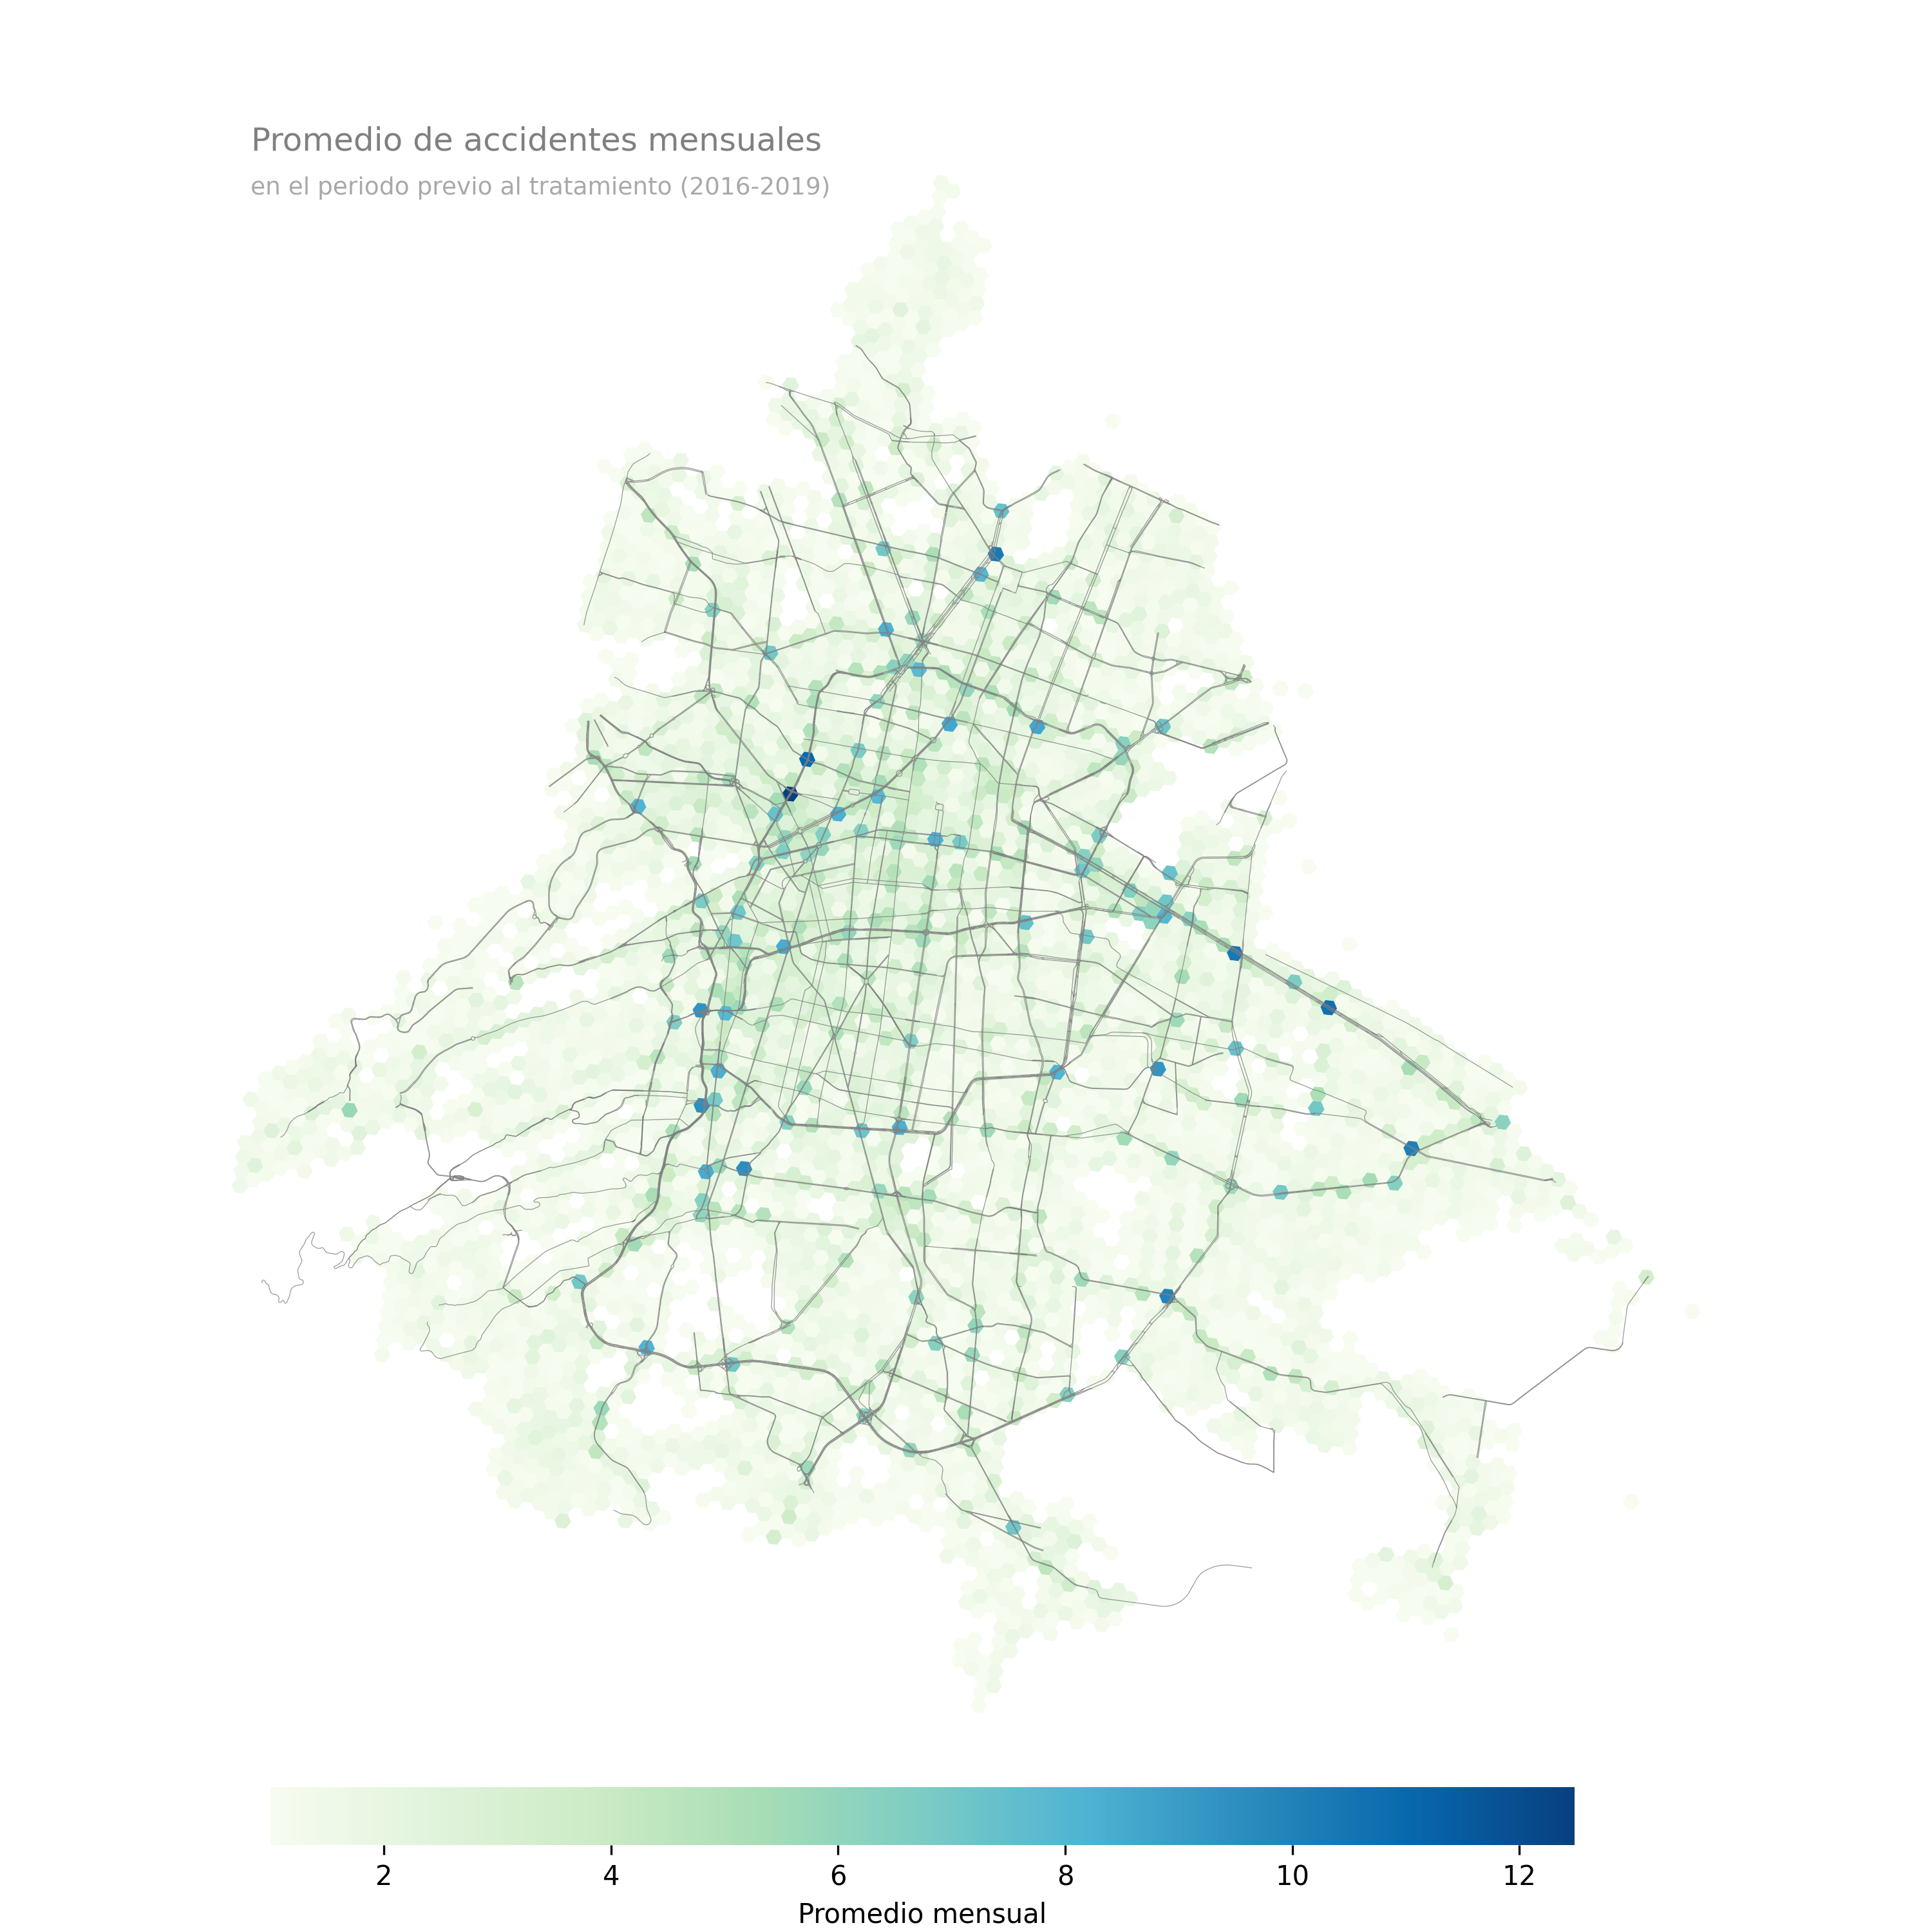
\includegraphics[width=1\linewidth]{Imagenes/promedio-accidenes-mensuales-pre-tratamiento-choroplet.png}
\end{figure}

\begin{figure}
    \centering
    \caption{Distribución de promedio de accidentes mensuales (2016-2019)}
    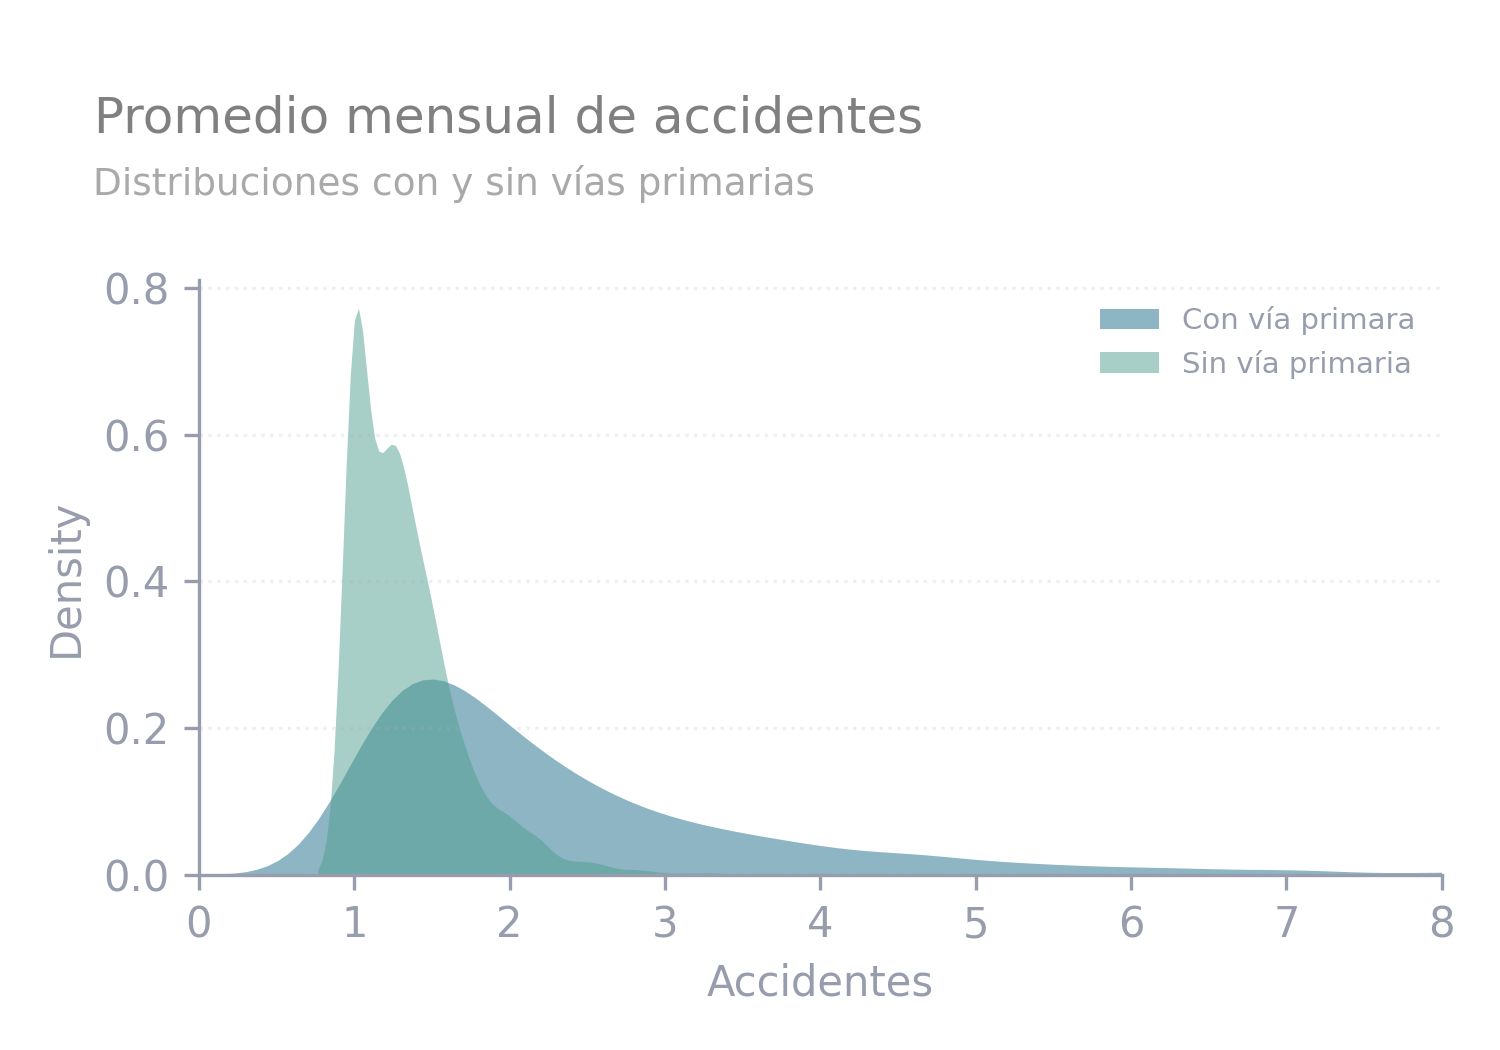
\includegraphics[width=.6\linewidth]{Imagenes/distribucion-promedio-mensual-accidentes-hexagonos.png}
\end{figure}

Por último, las zonas con vías primarias tienden a presentar un perfil de uso de suelo distinto. Para aproximar la intensidad de actividad comercial y de servicios, utilizo la API de \emph{Places Aggregate} de Google para obtener el número de establecimientos por hexágono (de la misma dimensión que el análisis de accidentes). Se diseñó una lista de categorías de lugares que ayudaran a tener una representación general de cada área \footnote{Lista de categorías utilizadas en la llamada a la API de Google Places Aggregate: \texttt{restaurant}, \texttt{cafe}, \texttt{shopping\_mall}, \texttt{supermarket}, \texttt{convenience\_store}, \texttt{grocery\_store}, \texttt{store}, \texttt{gas\_station}, \texttt{bank}, \texttt{atm}, \texttt{hospital}, \texttt{pharmacy}, \texttt{school}, \texttt{gym}, \texttt{night\_club}, \texttt{transit\_station}, \texttt{bus\_station}, \texttt{subway\_station}.}. En promedio, los hexágonos con vías primarias concentran $77.79$ establecimientos (desviación estándar $69.10$), mientras que los hexágonos sin vías primarias tienen en promedio $56.85$ establecimientos (desviación estándar $63.36$). Si bien la variabilidad es alta y la mayor concentración de negocios se observa en torno al centro de la ciudad, existe una diferencia promedio consistente entre ambos tipos de zonas.\\

\begin{figure}
    \centering
    \caption{Distribución de promedio de accidentes mensuales (2016-2019)}
    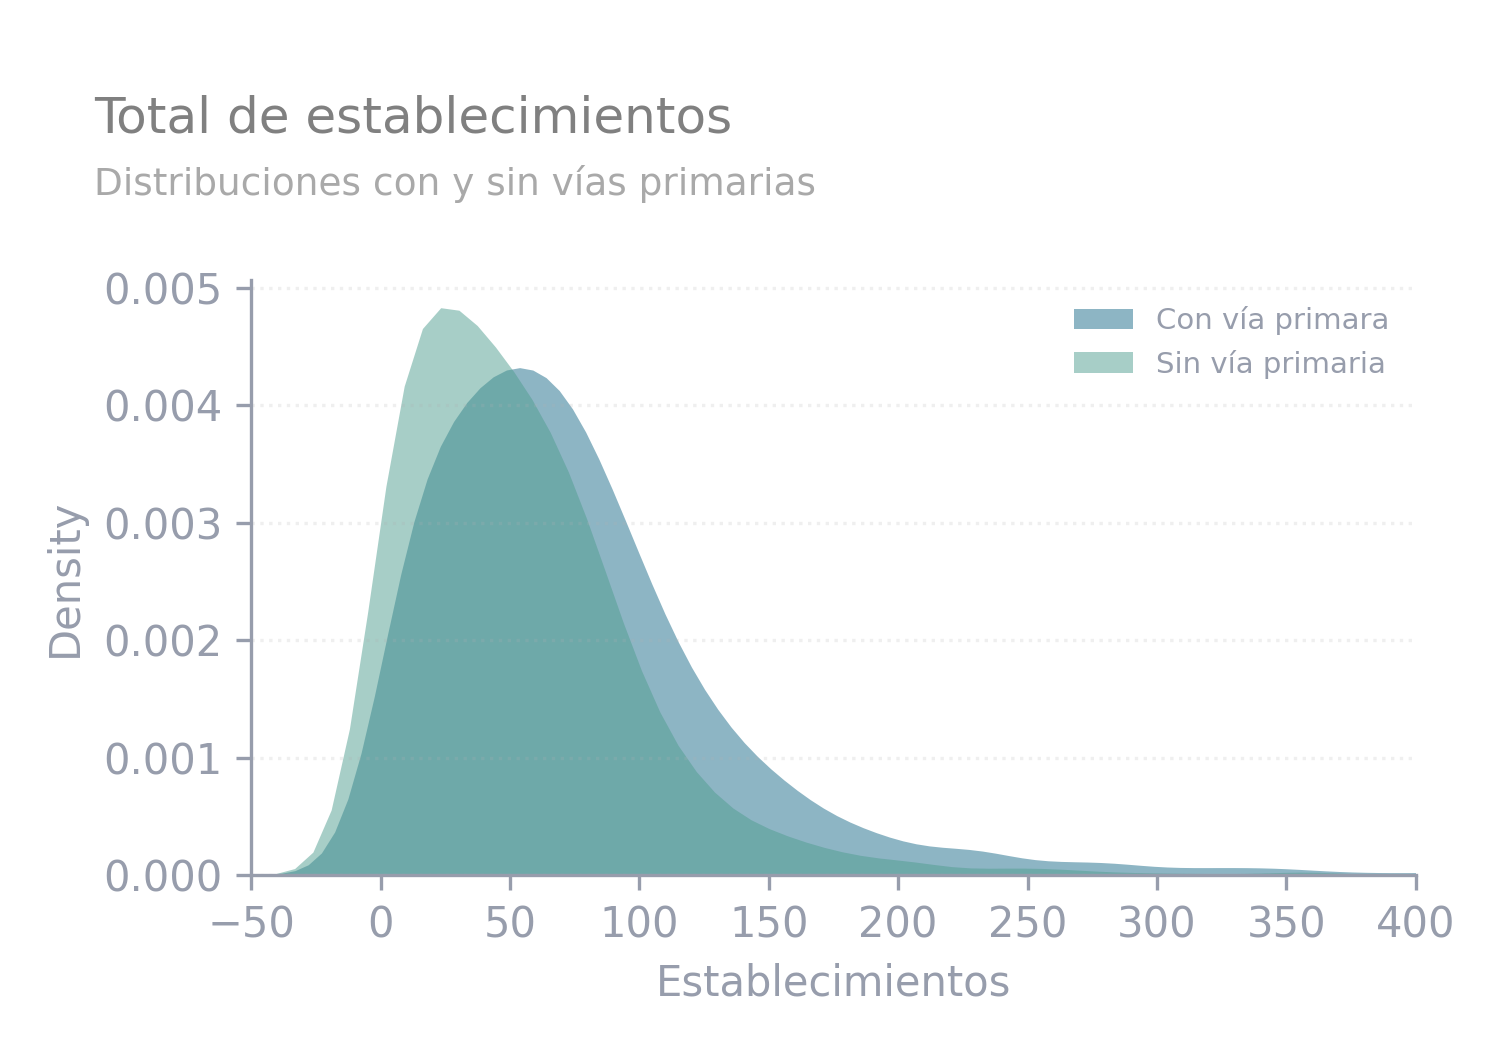
\includegraphics[width=.6\linewidth]{Imagenes/distribucion-establecimientos-cdmx-hexagonos.png}
\end{figure}

\begin{figure}
    \centering
    \caption{Establecimientos en la CDMX}
    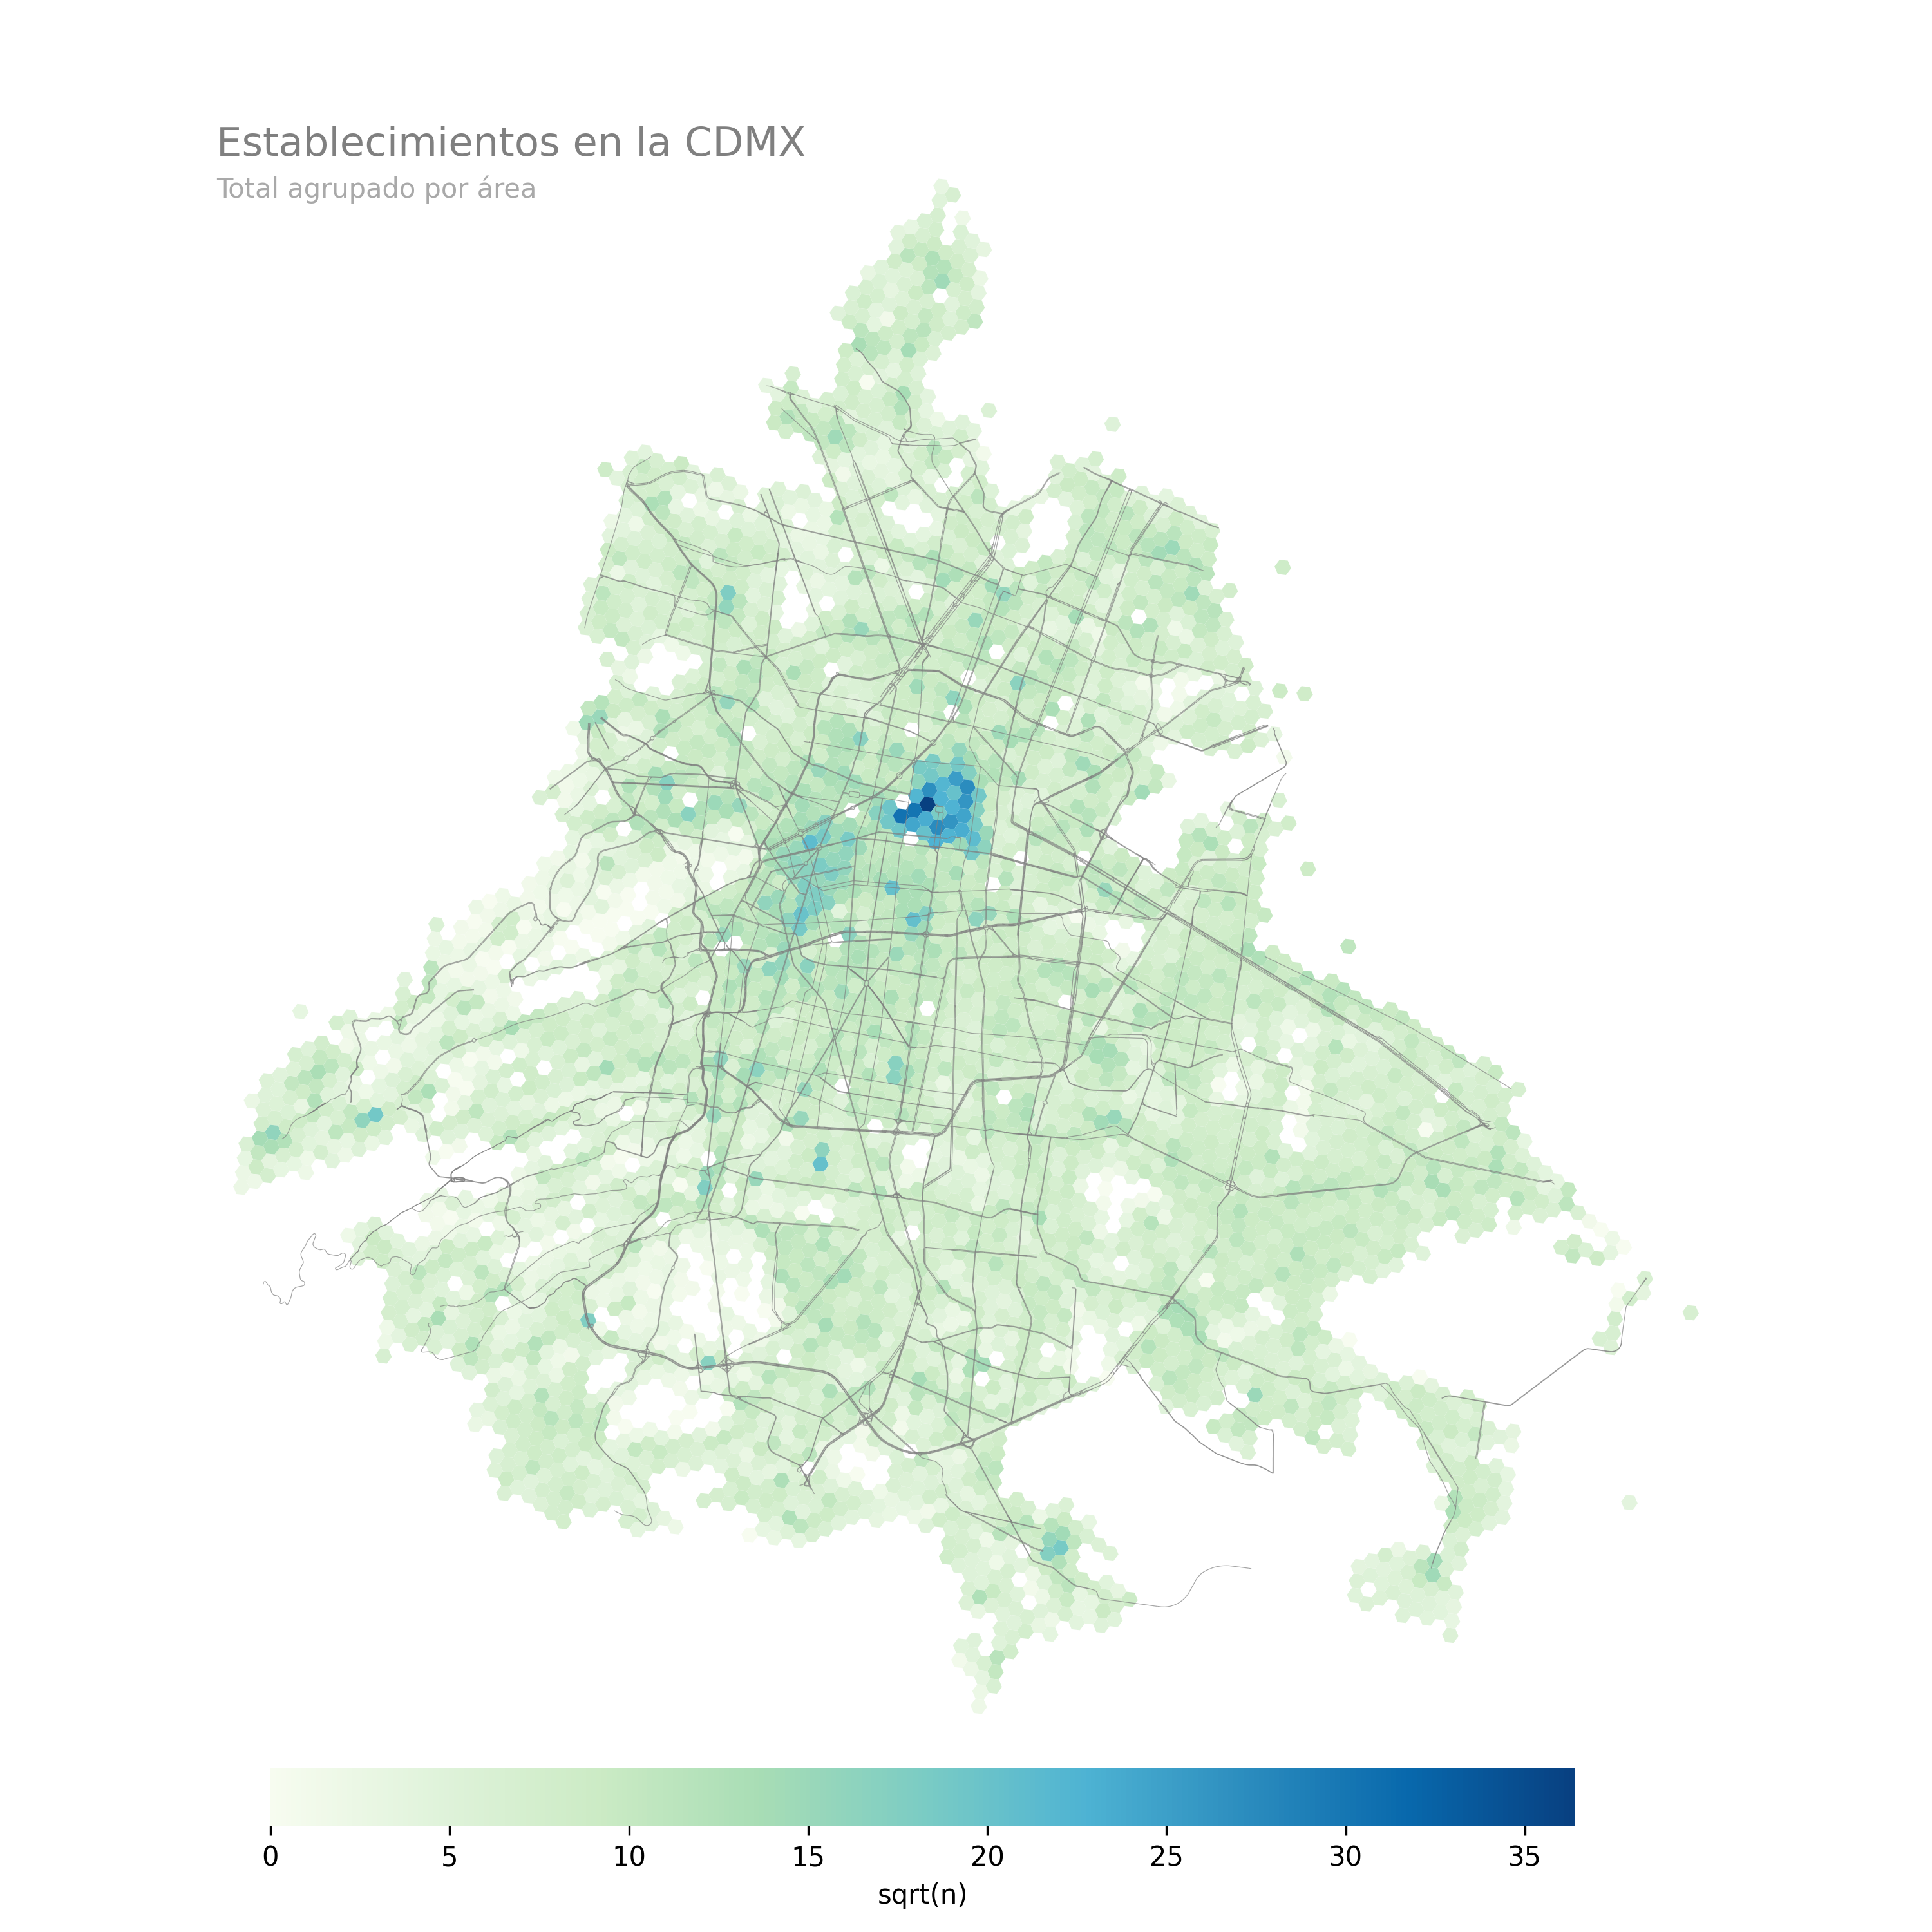
\includegraphics[width=1\linewidth]{Imagenes/establecimientos-en-la-cdmx.png}
\end{figure}
En conjunto, estas diferencias en velocidad reglamentaria, siniestros y nivel de actividad económica muestran que las zonas con y sin vías primarias corresponden a entornos viales y urbanos cualitativamente distintos. Una comparación directa entre ellas introduciría sesgos difíciles de manejar, incluso tras ajustar por covariables observables. Por este motivo, acoto el universo de análisis a las áreas —tratadas y de control— definidas por la malla de círculos alrededor de las cámaras que, además, presentan traslape con al menos una vía primaria de la Ciudad de México. Con base en este universo más homogéneo, en la siguiente sección implemento un procedimiento de emparejamiento por puntaje de propensión, cuyo propósito es hacer más creíbles las comparaciones causales entre áreas tratadas y de control.

\section{Estrategia de identificación}
\noindent El objetivo de esta tesis es estimar el efecto causal de la instalación de cámaras de velocidad sobre la seguridad vial en su entorno inmediato. En particular, me interesa cuantificar cómo cambia, en las áreas donde se colocaron radares, el promedio mensual de accidentes por nivel de severidad y la tasa promedio mensual de accidentes, en comparación con lo que hubiera ocurrido en ausencia de cámaras. En términos de inferencia causal, este efecto se interpreta como un \emph{average treatment effect on the treated} (ATT): el efecto promedio de contar con cámara sobre las áreas efectivamente tratadas, tomando como contrafactual áreas de control emparejadas que comparten características observables similares.\\

Dada la naturaleza panel de la base de datos y el hecho de que el programa de fotocívicas se implementó simultáneamente para todas las cámaras el 22 de abril de 2019, la estrategia principal de estimación se basa en modelos de diferencia en diferencias con efectos fijos. La unidad de observación es el área de análisis (círculo tratado o de control) en cada periodo, y el modelo incluye efectos fijos por unidad y por mes, de modo que se controlan tanto las características invariables en el tiempo de cada área como los choques comunes a toda la ciudad en cada periodo. El coeficiente de interés es el de la interacción entre una dummy de tratamiento (área con cámara) y una dummy de periodo posterior a la entrada en vigor del programa; este parámetro captura el cambio diferencial en los resultados de seguridad vial en áreas tratadas frente a sus controles después de la instalación de las cámaras.\\

Existen, en principio, varias formas alternativas de aproximarse a este problema. Una opción natural sería un ejercicio tipo \emph{before--after} en las áreas donde se instalaron las cámaras, comparando directamente el nivel de siniestros antes y después de abril de 2019. Sin embargo, esta aproximación es especialmente problemática en este contexto por dos razones. Primero, el periodo de estudio incluye el choque exógeno de la pandemia de COVID-19, que alteró de manera drástica los patrones de movilidad y, por tanto, la siniestralidad vial. Un simple \emph{before--after} confundiría los efectos de la pandemia con los del programa de fotocívicas. Segundo, incluso en ausencia de la pandemia, cualquier cambio en tendencias generales de accidentes en la ciudad podría ser erróneamente atribuido a las cámaras si no se cuenta con un grupo de comparación adecuado.\\

Otra alternativa sería estimar un modelo de diferencia en diferencias utilizando como controles todas las áreas elegibles que no recibieron cámaras. Sin embargo, como se discutió en la sección anterior, la asignación del programa no fue aleatoria: por diseño, las cámaras se instalaron en zonas con mayor riesgo vial. Usar de manera indiscriminada todas las demás áreas como contrafactual heredaría este sesgo de selección y llevaría a comparar zonas sistemáticamente más peligrosas con otras estructuralmente distintas, incluso si se controla por algunas covariables en la regresión. Bajo estas condiciones, el supuesto de independencia condicional resulta poco creíble.\\

También es conceptualmente posible apoyarse únicamente en \emph{propensity score matching} (PSM), emparejando cada área tratada con una o varias áreas de control similares en sus covariables pretratamiento y estimando el efecto como el promedio de las diferencias en los resultados. No obstante, el tratamiento aquí no es un evento puntual observado una sola vez, sino una intervención permanente a partir de una fecha concreta. En este marco, la estructura temporal contiene información valiosa que se desperdiciaría si se redujera el análisis a un comparativo estático entre tratadas y controles. Por ello, resulta más natural combinar el emparejamiento con un modelo de diferencia en diferencias.\\

En esta tesis, la estrategia de identificación combina precisamente ambas herramientas: primero, utilizo el \emph{propensity score} para construir pares de áreas tratadas y de control que sean lo más comparables posible en términos de covariables observables; después, aplico sobre esta muestra emparejada una regresión de diferencia en diferencias con efectos fijos por unidad y por mes. De esta manera, el \emph{matching} actúa como un paso de preprocesamiento que mejora la calidad del grupo de comparación, mientras que la estructura panel permite aislar cambios diferenciales en el tiempo asociados a la implementación del programa.\\

La probabilidad que se modela en el paso de PSM es la probabilidad de que un área determinada cuente con una cámara de velocidad condicional en las covariables observables seleccionadas. Para ello, estimo un modelo logístico en el que la variable dependiente es una dummy de tratamiento (presencia de cámara) y los regresores incluyen las características del entorno vial y urbano disponibles en el periodo pretratamiento. El \emph{propensity score} resume así, en una sola dimensión, la información relevante de las covariables utilizadas para la asignación del programa.\\

A partir de estos puntajes de propensión, implemento un esquema de \emph{nearest neighbor matching} 1:1 sin reemplazo. Es decir, para cada área tratada se selecciona como control aquella área sin cámara cuyo \emph{propensity score} presenta la menor diferencia absoluta respecto al de la unidad tratada, y cada área de control se utiliza a lo más una vez. Opto por el emparejamiento 1:1 sin reemplazo por dos motivos. Primero, garantiza que cada unidad de control emparejada representa un contrafactual razonablemente cercano en términos de probabilidad de tratamiento, en lugar de reutilizar en exceso un pequeño conjunto de controles “muy buenos”, lo que concentraría la inferencia en pocas zonas de la ciudad. Segundo, en las pruebas de balance, esta configuración produjo la mejor combinación entre similitud de covariables y tamaño efectivo de la muestra: al intentar emparejar más de un control por tratada se incrementaba el ruido, pues necesariamente se incorporaban pares con diferencias más grandes en el \emph{propensity score}.\\

Un requisito central de esta estrategia es el supuesto de \emph{common support}: para cada valor del \emph{propensity score} observado en las áreas tratadas debe existir un conjunto suficiente de áreas de control con valores similares. Más adelante, en la sección de balance, muestro la distribución de los puntajes de propensión para unidades tratadas y de control y verifico que, en términos generales, existe un traslape amplio entre ambos grupos. No obstante, en algunos radios fue necesario restringir la muestra y excluir ciertas áreas tratadas ubicadas en zonas del puntaje de propensión con muy poca densidad de controles comparables. Este recorte permite que el emparejamiento se realice únicamente en la región donde la comparación entre tratadas y controles resulta defendible.\\

La calidad del emparejamiento se evalúa mediante la \emph{standardized mean difference} (SMD) para cada covariable incluida en el modelo de \emph{propensity score}. Reporto los valores de SMD antes y después del \emph{matching} y utilizo como referencia el criterio usual de considerar aceptable un desbalance inferior a 0.1 en valor absoluto. Si bien no todas las covariables alcanzan exactamente ese umbral, los desbalances residuales son pequeños y se reducen de manera sustancial respecto a la muestra original. Esto indica que, después del emparejamiento, las distribuciones de las covariables observables en los grupos tratado y de control son muy similares.\\

Una vez construido el conjunto de pares tratada–control, estimo el efecto de las cámaras mediante una regresión de diferencia en diferencias, utilizando como unidades tratadas las áreas con radares de velocidad y como controles sus respectivos \emph{matches}. Dado que el emparejamiento ya garantiza un alto grado de similitud en las covariables observables pretratamiento, especifico el modelo de diferencia en diferencias únicamente con efectos fijos por unidad y por mes, sin añadir controles adicionales. La inclusión de efectos fijos por área captura diferencias invariables en el tiempo entre cada par tratada–control, mientras que los efectos fijos temporales recogen shocks comunes (incluido el choque de la pandemia) que afectan de manera similar a todas las áreas en un mismo periodo. Bajo el supuesto estándar de tendencias paralelas entre los grupos emparejados, el coeficiente de la interacción tratamiento–periodo posterior puede interpretarse como el efecto causal promedio de las cámaras sobre los resultados de seguridad vial en las áreas tratadas.\\

Esta combinación también vuelve más creíble la comparación entre áreas tratadas y de control. Dado que las cámaras se reubicaron hacia zonas con mayor riesgo, no basta con comparar cualquier vialidad con cámara contra cualquier vialidad sin cámara. El emparejamiento permite partir de áreas observacionalmente similares, y la diferencia en diferencias aprovecha esa base para aislar mejor los cambios posteriores a la implementación del programa.

\noindent A partir de esta discusión conceptual, en esta sección presento la evidencia empírica que utilizo para evaluar qué tan aceptable es ese supuesto en la muestra emparejada. La verificación se apoya en dos pruebas complementarias. La primera es una inspección visual de las trayectorias pevias al tratamiento. Para ello, construyo gráficas de tendencias mensuales promedio para los distintos radios evaluados, comparando en cada caso las áreas tratadas con: (i) todos los controles elegibles y (ii) los controles emparejados por \emph{propensity score}. Hago uso de tres años de información previos a la implementación y tres años posteriores, y se realiza para el total de accidentes y para cada nivel de severidad (\emph{MIN}, \emph{PIC} y \emph{FCS}). En la muestra sin emparejar, las áreas tratadas presentan de manera sistemática niveles promedio de siniestralidad más altos, algo consistente con el sesgo de selección que motivó el uso de PSM. Aun así, en términos generales las trayectorias previas ya lucen parecidas. Después del emparejamiento, el traslape entre curvas aumenta de forma importante: no solo se reducen las diferencias de nivel, sino que las tendencias se vuelven mucho más similares. Las series de accidentes fatales son más ruidosas, algo esperable dada la baja frecuencia de estos eventos. El caso donde todavía se aprecia una diferencia más visible es el de accidentes menores en el radio de 50 metros, donde alrededor de año y medio antes de la intervención persiste una ligera discrepancia; aun así, esa diferencia es menor que la observada en la muestra original. La figura siguiente muestra precisamente ese radio.\\

\begin{figure}[htbp]
    \centering
    \caption{Tendencias promedio mensuales de accidentes en radios de 50 metros, con y sin matching}
    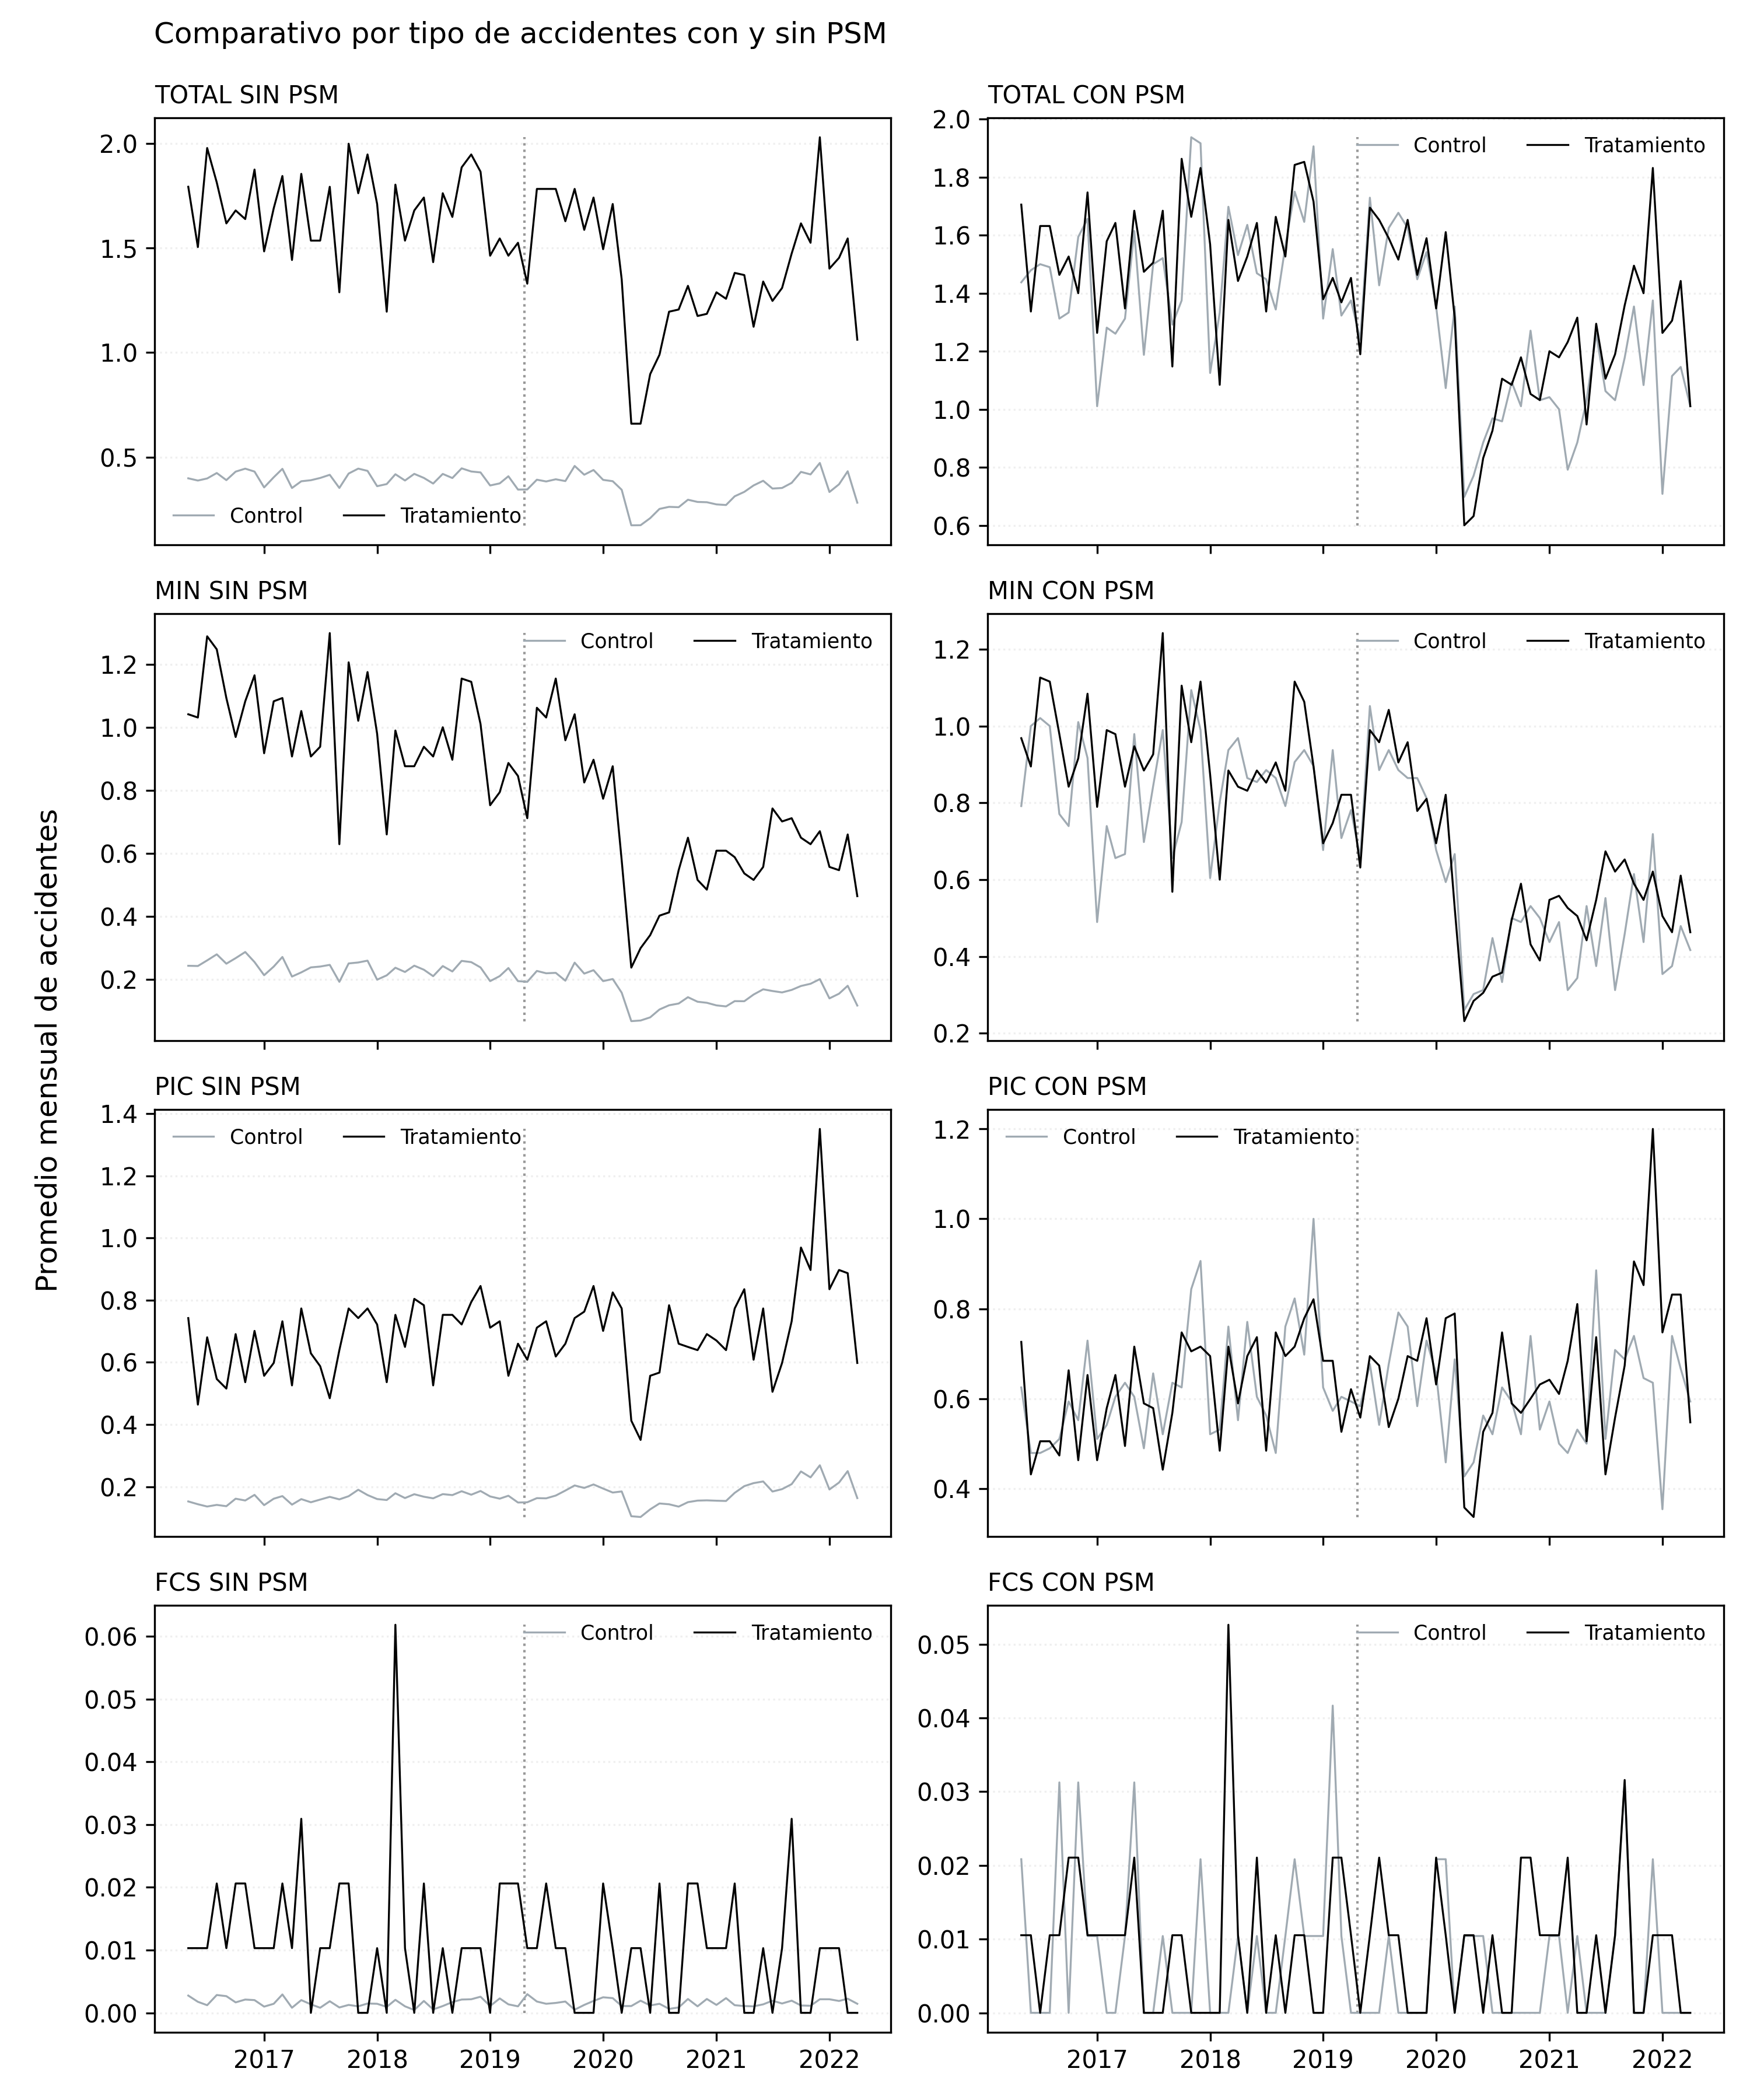
\includegraphics[width=\textwidth]{Imagenes/mean_accidents_trends/trend_mean_accidents_50.png}
\end{figure}

La segunda evaluación consiste en pruebas placebo usando exclusivamente los tres años previos al inicio del programa. Para ello, vuelvo a estimar la especificación principal sobre la misma muestra emparejada, pero asignando fechas ficticias de tratamiento a 18, 12 y 6 meses antes de la implementación real. Lo que esperaríamos es lo siguiente: si el modelo estuviera detectando diferencias previas entre tratados y controles, deberían aparecer coeficientes significativos incluso antes de que el programa comenzara. En total, se estiman 144 coeficientes para los distintos radios, variables de resultado y ventanas placebo. De ellos, 143 no son estadísticamente significativos. La única excepción aparece en la tasa de accidentes menores para el radio de 50 metros cuando la fecha de prueba se ubica 18 meses antes del inicio del programa, con significancia al 95\%. Estos resultados son consistentes con el supuesto de tendencias paralelas, aunque sugieren interpretar con un poco más de cautela esa especificación puntual.\\

La evidencia presentada no permite probar de forma definitiva el supuesto de tendencias paralelas, algo que además no es posible hacer de manera directa. Sin embargo, sí aporta elementos a favor de su plausibilidad. En especial, una vez construido el grupo de control mediante \emph{propensity score matching}, las áreas tratadas y sus controles emparejados muestran trayectorias antes del tratamiento que son similares y, salvo una excepción aislada, no presentan efectos placebo previos a la implementación del programa. En este sentido, la evidencia respalda la interpretación del coeficiente de diferencia en diferencias como una aproximación al efecto causal de las cámaras sobre la siniestralidad vial.\\

Finalmente, una ventaja adicional de esta estrategia es su interpretabilidad y capacidad de replicación. Al partir de una comparación explícita entre áreas tratadas y controles muy similares, y estimar un efecto promedio bien definido sobre las unidades tratadas, los resultados pueden traducirse directamente en recomendaciones de política. En particular, si se encuentra que las cámaras reducen de manera significativa la frecuencia o la severidad de los accidentes en su entorno inmediato, el mismo procedimiento de emparejamiento puede utilizarse en una segunda etapa para identificar qué otras áreas de la ciudad presentan perfiles de riesgo y características viales similares a las zonas tratadas actuales. Estas áreas serían candidatas naturales para una eventual expansión del programa de fotocívicas, manteniendo la lógica de focalizar la intervención donde los beneficios esperados sean mayores.\\ 
